\section{Mathematical Context and Background}
\label{sec:review}

In order to provide some mathematical context for our correlation model
developments, we first outline the generic inverse problem that is central to
a variety of applications such as numerical weather prediction and state
estimation.
Our notation closely follows \citet{ide_unified_1997}, and we note that matrix
notation is used to describe the problem, but these matrices are never formed
explicitly.
Rather, all matrices presented can be described as operators that can be applied
scalably in high dimensional inverse problems.
We then review correlation models that are based on the application of a
diffusion operator \citep{weaver_correlation_2001,mirouze_representation_2010},
which are commonly used for large scale geophysical inverse problems
\citep[e.g.][]{forgetECCOv4}.
We then discuss the developments from \citet{RSSB:RSSB777}, outlining the
connection between the solution to a Stochastic PDE (SPDE) and a Gaussian random
field with Mat\'ern type covariance.
We finish by showing a comparison of auto-regressive and the more general
Mat\'ern type correlation functions with a classical Gaussian in order to
further motivate our development of an anistropic, nonstationary correlation
model which is presented in \cref{sec:matern_operator}.


\subsection{Inverse Problem Formulation}
\label{ssec:da_formulation}

We consider the general problem of finding the optimal control vector,
$\params$, which minimizes the regularized model-data misfit cost function
\begin{linenomath*}\begin{equation*}
    \cf(\params) =
        \dfrac{1}{2}||\pto(\params) - \data||_{\obsCovMat^{-1}}^2
        +
        \dfrac{1}{2}||\params - \priorParams||_{\priorCovMat^{-1}}^2 \, .
\end{equation*}\end{linenomath*}
Here $\norm{\mathbf{v}}_A = \sqrt{\mathbf{v}^T A \mathbf{v}}$ is a weighted
Euclidean norm.
The solution to this inverse problem, $\paramsMAP$, arises from a tradeoff between fitting the
observational data, $\data$, via the observation operator, $\pto(\cdot)$,
and minimizing deviations from the background-state $\priorParams$.
This tradeoff is governed by the two error covariances, $\obsCovMat$ and
$\priorCovMat$, which dictate how much deviation is acceptable in either term.
On the one hand, the observational error covariance matrix
$\obsCovMat$ represents our uncertainty
in the observational data, together with our confidence in the model's ability
to represent the observed values.
On the other hand, the background-state covariance matrix $\priorCovMat$
represents our uncertainty in the prior estimate or background state,
$\priorParams$.

To be explicit, we focus on how our correlation model fits into the
background-state error covariance, $\priorCovMat$.
However, we note that the formulation could be used for specifying correlations
between observations in a similar fashion to \citet{guillet_modelling_2019}, but
we leave this for future investigation.
In the general case, the control vector $\params$ could be multivariate,
including initial conditions of the system state, uncertain boundary
conditions, or uncertain parameter fields.
Here we employ the decomposition proposed by
\citet{derber_reformulation_1999}
in order to separate the multivariate (i.e.\ cross-variable)
covariance relationships from the univariate (i.e.\ assumed
independent) covariance relationships.
Specifically, the background-state covariance is decomposed as follows
\begin{linenomath*}\begin{equation*}
    \priorCovMat \coloneqq \balanceOperator\unbalancedPriorCovMat\balanceOperator^T \,
    ,
\end{equation*}\end{linenomath*}
where $\balanceOperator$ is a balance operator that deals with the
cross-variable correlations.
The matrix $\unbalancedPriorCovMat$ describes the covariance for the unbalanced
variables and has a block-diagonal structure, such that each
covariance is described independently.
The unbalanced covariance is further factored as
\begin{linenomath*}\begin{equation*}
    \unbalancedPriorCovMat \coloneqq \Sigma \mathcal{C} \Sigma
\end{equation*}\end{linenomath*}
where $\Sigma$ is a diagonal scaling matrix, containing the desired pointwise
standard deviation values and $\mathcal{C}$ is a block diagonal correlation matrix,
describing each variable's independent correlation structure.
To be concrete, this can be viewed as
\begin{linenomath*}\begin{equation*}
    \unbalancedPriorCovMat =
    \begin{pmatrix}
        \Sigma_\alpha\corrMat_\alpha\Sigma_\alpha & 0 & \cdots & 0 \\
        0 & \Sigma_\beta\corrMat_\beta\Sigma_\beta & \cdots & 0 \\
        0 & 0 & \ddots & 0  \\
        0 & 0 & \cdots & \Sigma_\gamma\corrMat_\gamma\Sigma_\gamma \\
    \end{pmatrix}
\end{equation*}\end{linenomath*}
where $\alpha, \beta, \gamma$ are placeholders for unique variables, and each
$\Sigma_\alpha, \corrMat_\alpha$ pair describes the amplitude of pointwise standard deviation
and spatial correlation for each variable.
The goal of this paper is to formulate a generic operator for $\corrMat$, or
more specifically for its square root $\corrMat^{1/2}$ such that $\corrMat =
\corrMat^{1/2}\corrMat^{T/2}$, that could be
used in a variational data assimilation system to specify $\corrMat_\alpha$,
$\corrMat_\beta$, etc.
To provide some additional context,
we first review past work that has achieved this with a generalized
diffusion-based operator.


\subsection{Diffusion Based Correlation Models}
\label{ssec:wc01_review}

A common method for specifying the correlation structure for
$\corrMat$ in variational data assimilation systems, especially in
oceanographic applications, is through the solution of a generalized diffusion
equation,
\begin{linenomath*}\begin{equation}
    \dfrac{\partial \uni}{\partial t} = \nabla \cdot \kappa \nabla\uni \, .
    \label{eq:diffusion}
\end{equation}\end{linenomath*}
Here $\kappa$ is a diffusion tensor that controls anisotropy and
nonstationarity, $t$ is a ``pseudo-time'' coordinate, and the solution to this
equation has a Gaussian, or ``Gaussian-like'', covariance.

Building on work from \citet{derber_global_1989, egbert_topexposeidon_1994,
bennett_generalized_1996},
\citet{weaver_correlation_2001} showed that an explicit, forward Euler solution to
\cref{eq:diffusion} provides a scalable approach to defining correlations in
complex domains.
That is, the solution $\uni(T)$ is given by forward pseudo-time stepping
\begin{linenomath*}\begin{equation}
    \uni(T) = \left( I + \nabla\cdot\kappa\nabla\right)^p \uni(t_0) \, ,
    \label{eq:wc01_diffusion}
\end{equation}\end{linenomath*}
or equivalently through the application of the Laplacian-like operator
$A_\text{ED} \coloneqq \left(I+\nabla\cdot\kappa\nabla\right)^p$, where $p$ is chosen in
order to achieve numerical stability \citep[see][for details regarding the
discretized form of this operator, and extensions of the model briefly shown
here]{weaver_correlation_2001}.
The solution $\uni(T)$ is shown to have an approximately Gaussian covariance
structure.
A correlation model is thus defined by estimating the pointwise
variance of $A_\text{ED}$, $\hat{\sigma}^2(\x)$, in order to define the normalization
matrix
\begin{linenomath*}\begin{equation*}
    \normalizer \coloneqq \text{diag}\{1/\hat{\sigma}_i\}_{i=1}^{\nuni} \, ,
\end{equation*}\end{linenomath*}
where we use $i$ to refer to each grid cell, such that the correlation matrix is
defined through its square root
\begin{linenomath*}\begin{equation}
    \corrMat^{1/2}_\text{ED} \coloneqq \normalizer A_\text{ED} \, .
\end{equation}\end{linenomath*}

The explicit diffusion-based correlation model as briefly summarized here
directly approximates a Gaussian structure.
However, a limitation of the explicit diffusion approach is that in some cases, many
iterations are required to keep the scheme stable (i.e.\ a large value of $p$ is
required in \cref{eq:wc01_diffusion}).
As such, \citet{mirouze_representation_2010} and
\citet{carrier_background-error_2010} developed correlation models based on the
\textit{implicit} solution of \cref{eq:diffusion}:
\begin{linenomath*}\begin{equation}
    \left( I - \nabla\cdot\kappa\nabla\right)^M\uni(T) = \uni(t_0) \, ,
    \label{eq:implicit_diffusion}
\end{equation}\end{linenomath*}
which is unconditionally stable.
In this case, a square-root correlation operator is defined through the
``implicit diffusion operator''
\begin{linenomath*}\begin{equation}
A_\text{ID} \coloneqq \left(I - \nabla \cdot \kappa\nabla\right)^{-M}
\end{equation}\end{linenomath*}
as
\begin{linenomath*}\begin{equation}
    \corrMat^{1/2}_\text{ID} \coloneqq \normalizer A_\text{ID} \, ,
\end{equation}\end{linenomath*}
with $\normalizer$ defined based on the operations that precede it.

\citet{mirouze_representation_2010} provide the theoretical underpinnings for
the implicit diffusion approach, and show details regarding its discretization
in general curvilinear coordinates.
Additionally, the authors show that this correlation model corresponds
with an $M$th order auto-regressive (AR) function,
which is a subclass of
Mat\'ern type correlation models \citep[see][for more description behind the
parameters controlling this model]{weaver_diffusion_2013}.
Thus, the correlation model has a more general shape, which in the limit of
$M\rightarrow\infty$, approaches a classical Gaussian structure (see
\cref{ssec:correlation_comparison}).

In this work, we formulate a correlation operator in a similar fashion by
directly parameterizing the
elliptic partial differential equation that corresponds to the more generic
Mat\'ern type correlation (or covariance) structure.
In the following subsections, we provide some background on this general correlation
structure to give our developments some context and motivation.

%is a normlization matrix filled with the pointwise inverse standard deviation of the
%operation $\left(I+\nabla\cdot\kappa\nabla \right)^p W^{-1/2}$.
%This definition ensures that the filter defined by $\corrMat^{1/2}_\text{WC01}$
%preserves variance.
%The tensor, $\kappa$, controls the correlation length scales imposed on the
%random field in question.
%Correlation length scales are isotropic (i.e.\ the same in all directions) and
%stationary (i.e.\ they do not change with spatial location) when $\kappa$ is
%constant such that
%\begin{linenomath*}\begin{equation*}
%    L^2 = 2\kappa T \, ,
%\end{equation*}\end{linenomath*}
%where $T\coloneqq p \Delta t$ is the total ``diffusion'' time and $L$ is the
%desired length scale.
%In general, the diffusion tensor can be formulated to produce anisotropic and
%nonstationary length scales, and applied to spherical domains.
%However, a few subtle issues arise in the numerical its implementation.
%First, the number of timesteps, $p$, required to integrate the diffusion
%equation for numerical stability is somewhat unclear.
%In WC01, a necessary but insufficient stability requirement
%$p > 2 (L/\Delta x)^2$ is given.
%However, in practice uncovering the true required value of $p$ requires some
%guess work, and in our experience is multiplicative factor of this lower bound
%(typically $\sim 3$ for our application).
%Additionally, adjoint-based data assimilation systems based on algorithmic
%differentiation may require additional storage, random access memory, or recomputations in order
%to keep track of intermediate results during the adjoint (i.e.\ reverse) timestepping
%in the diffusion model.
%
%In this work we formulate an operator for $\corrMat_\alpha$ which bypasses these
%issues entirely.
%First, we avoid the issue of having to guess the required time steps for numerical
%stability because the application of our correlation operator amounts to solving an
%elliptic PDE, for which a tolerance can be prescribed more readily.
%Moreover, we show that for practical applications this tolerance can be reliably
%prescribed to be quite high $\bigo(10^{-2})$, such that solving the required
%elliptic PDE is computationally efficient.
%Finally, the operator is self-adjoint and so implementing the covariance model
%within any adjoint based solver is a nonissue.
%To provide some details, we next outline the basis for this Mat\'ern covariance
%model from \citet{RSSB:RSSB777}.


\subsection{Review of the Mat\'ern Correlation Structure}
\label{ssec:matern_review}

In this section we review the link between an elliptic stochastic partial
differential equation (SPDE) and Gaussian random fields.
The Mat\'ern covariance function between two points, $\xh_1,\xh_2\in\defdomain =
\ndspace$ can be expressed as:
\begin{linenomath*}\begin{equation}
    c(\xh_1,\xh_2) = \dfrac{\hat{\sigma}^2}{2^{\meandiff-1}
    \mathcal{G}(\meandiff)}
    \Big(\sqrt{\deltah} ||\xh_2-\xh_1||\Big)^\meandiff
    \mathcal{B}_\meandiff
    \Big(\sqrt{\deltah} ||\xh_2-\xh_1||\Big) \, .
    \label{eq:matern_covariance_iso}
\end{equation}\end{linenomath*}
Here
$\mathcal{G}$ is the Gamma function,
$\mathcal{B}_\meandiff$ is the modified
Bessel function of the second kind and order $\meandiff$,
$\deltah>0$ is a scaling parameter, and $\meandiff>0$
controls the mean-square differentiability of the underlying statistical process
described by the Mat\'ern covariance.
We note that in the limit of $\meandiff\rightarrow\infty$, the Mat\'ern-type
covariance becomes a classical Gaussian.
Throughout, we refer to a ``Mat\'ern field'' as any normally distributed field that has
covariance described by the Mat\'ern covariance function,
\cref{eq:matern_covariance_iso}.
Additionally, we note that this analytical function only pertains to fields where the
assumptions of stationarity (i.e.\ no spatial dependence) and isotropy (i.e.\ no
directional dependence) hold, and we use notation with ``hats'' $(\hat{\cdot})$
when this is the case.
The marginal variance of such a Mat\'ern field has the analytical form
\begin{linenomath*}\begin{equation}
    \hat{\sigma} = \dfrac{\mathcal{G}(\meandiff)}{
        \mathcal{G}(\meandiff + \materndim/2)(4\pi)^{\materndim/2}
        \deltah^\meandiff
    } \, ,
    \label{eq:matern_variance}
\end{equation}\end{linenomath*}
and thus the Mat\'ern covariance can be described via a correlation
function, $r(\xh_1, \xh_2)$, that is scaled by the marginal variance:
\begin{linenomath*}\begin{equation}
    c(\xh_1, \xh_2) = \hat{\sigma}\,r(\xh_1, \xh_2) \, .
\end{equation}\end{linenomath*}

The key relationship discussed in \citet{RSSB:RSSB777} is that any solution to
the elliptic SPDE,
\begin{linenomath*}\begin{equation}
    \Big(\deltah - \nablah\cdot\nablah\Big)^{M}\hat{\uni}(\xh) =
    \Wh(\xh) \, ,
    \label{eq:spde_iso}
\end{equation}\end{linenomath*}
is a Mat\'ern field.
Here
$\Wh$ is a white noise process defined on the space $\defdomain$ and
\begin{linenomath*}\begin{equation}
    M = \meandiff/2 + \materndim/4
    \label{eq:meandiff}
\end{equation}\end{linenomath*}
The original connection between the Mat\'ern covariance function and solutions
to \cref{eq:spde_iso} was proven by
\cite{whittle_stationary_1954,whittle1963stochastic}, who
used the spectral properties of the operator $(\deltah -
\nablah\cdot\nablah)^M$ to show that Mat\'ern fields are the only
stationary solutions to \cref{eq:spde_iso}.
The result shown in \citet{RSSB:RSSB777} is
that there is an explicit link between discrete solutions to
\cref{eq:spde_iso} for any triangulation or rectangular lattice of $\ndspace$
and Mat\'ern class Gaussian fields.
More importantly, \citet{RSSB:RSSB777} showed that the SPDE form allows
one to easily describe Gaussian fields with nonstationary and anisotropic covariance structures.
For instance, by allowing the parameter $\deltah$ to vary in space, the solution
becomes nonstationary and the analytical Mat\'ern covariance applies locally.

Within this work, we suggest to define a correlation operator through the
elliptic operator in \cref{eq:spde_iso}.
For an isotropic and stationary case, the operator would be defined as
\begin{linenomath*}\begin{equation}
    \corrMat^{1/2}_\text{iso,stat} = \normalizer \left(\deltah -
    \nablah\cdot\nablah\right)^{-M} \, ,
    \label{eq:matern_corr_isostat}
\end{equation}\end{linenomath*}
with $\normalizer$ appropriately defined, but we extend this to a more general
case in \cref{sec:matern_operator}.


\subsection{Comparing the Mat\'ern and Auto-Regressive Functions}
\label{ssec:correlation_comparison}

To first provide some motivation behind our developments of the Mat\'ern
correlation function, we compare its structure to an AR function.
\cref{fig:correlation_comparison}(a) shows a comparison of these 1D correlation
structures as a function of distance, where each use a representative length
scale of $\rangeh = 4$.
Note that this is equivalent to setting $L=2$ for the length scale in
\citet{mirouze_representation_2010} (see definitions in Table 1).
The Mat\'ern function and Gaussian consistently reach an approximate correlation
of 0.14 when distance is equal to $\rangeh$.
The consistency here makes using the Mat\'ern correlation structure intuitive in
practice: no matter what value of $M$ (or alternatively $\meandiff$, see
\cref{eq:meandiff}), we can expect this approximate relationship to hold.


\begin{figure}
    \centering
    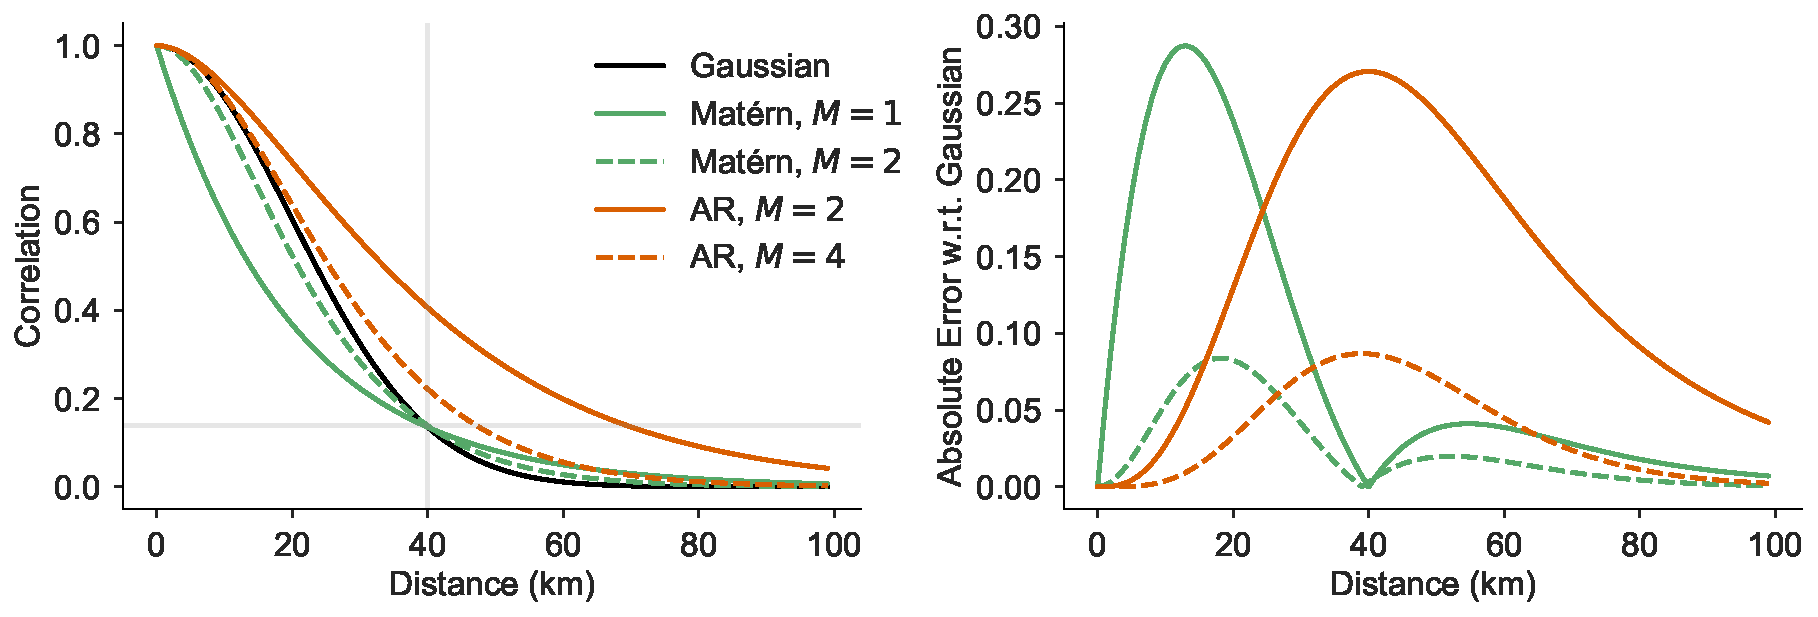
\includegraphics[width=\textwidth]{../figures/correlation_comparison.pdf}
    \caption{(a) Correlation as a function of distance given by
        Mat\'ern (green; \red{EQN}),
        auto-regressive (AR; orange),
        and Gaussian (black) functions.
        For each, we choose a length scale of $\rangeh = 4$, noting for
        comparison purposes that this corresponds to $L=2$ using the notation in
        \citet{mirouze_representation_2010}.
        (b) Absolute error considering the difference between the Mat\'ern and
        AR functions with respect to a Gaussian with the same length scale.
    }
    \label{fig:correlation_comparison}
\end{figure}

Additionally, \cref{fig:correlation_comparison}(b) shows the error in each
Mat\'ern and AR functions relative to a Gaussian.
We note that we get similar levels of error between the two when $M$ is half for
the Mat\'ern function compared to the AR function.
This has practical implications, since in both cases $M$ corresponds to the
number of inverse elliptic operator applications required for achieving a
correlation operator via the implicit diffusion approach (AR) or the approach
proposed here (Mat\'ern).
Thus, if the goal is to approximate a Gaussian, then using the direct Mat\'ern
shape results in half the required inverse elliptic solves.
However, we also stress that the desired shape of the correlation function will
be application dependent, and so we present a comparison from which
practitioners can take their pick.
